%% LaTeX2e class for student theses
%% sections/proposal.tex
%% 
%% Karlsruhe Institute of Technology
%% Institute for Program Structures and Data Organization
%% Chair for Software Design and Quality (SDQ)
%%
%% Dr.-Ing. Erik Burger
%% burger@kit.edu
%%
%% Version 1.3.6, 2022-09-28

\chapter{Secure Computation Platform Proposal}
\label{ch:proposal}

\section{Trust Model}
\label{sec:trust-model}

\todo[inline]{Explain needed services}

\subsection{Chain of Trust}

\todo[inline]{Trust Model: Chain of Trust}

\subsection{Roles}

\subsubsection*{Infrastructure Provider}

The infrastructure provider is responsible for the availability of the
infrastructure used to provide compute, networking, and storage resources. As
such the infrastructure controls and has access to the physical hardware and
firmware.

\subsubsection*{Service Provider}

The service provider is responsible for managing services that utilize the
infrastructure provided by the infrastructure provider in order to ease the
development and deployment of workloads. As such the service provider is not
only responsible for deploying the applications, but also to provide services
that allow the retrieval of attestation evidence and initialize TEE
environments.

It may be the case that the service and infrastructure provider roles are
aggregated into the same entity. As the attestation evidence is produced and
signed by the hardware vendor grouping these two roles does not affect the trust
model.

\subsubsection*{Application Owner}

The application owner designs and implements application workloads that will be
deployed and orchestrated by the service provider. This role needs to prove to
the customer aspects of compliance to the defined requirements. As such the
application owner has to provide TEE initialization images and attestation
verification services, or designate a trusted party to do so.

The application owner and service provider role should not be taken on by the
same entity, as the verification of the TEE provided by the service provider is
a responsibility of the application owner. Otherwise, the attestation results
can not be trusted.

\subsubsection*{Data Owner}

As the owner of the data used and manipulated by the application, this role is
concerned with the visibility, integrity of their data and the compliance of the
application with the requested requirements.

\subsubsection*{Verifier}

In order to remove the trust in the service provider an external party has to
verify the service providers' confidentiality claims. The verifier provides an
attestation service that appraises evidence and returns attestation results.

\section{Architecture}
\label{sec:proposal:architecture}

\subsection{Overview}

\begin{figure}
  \centering
  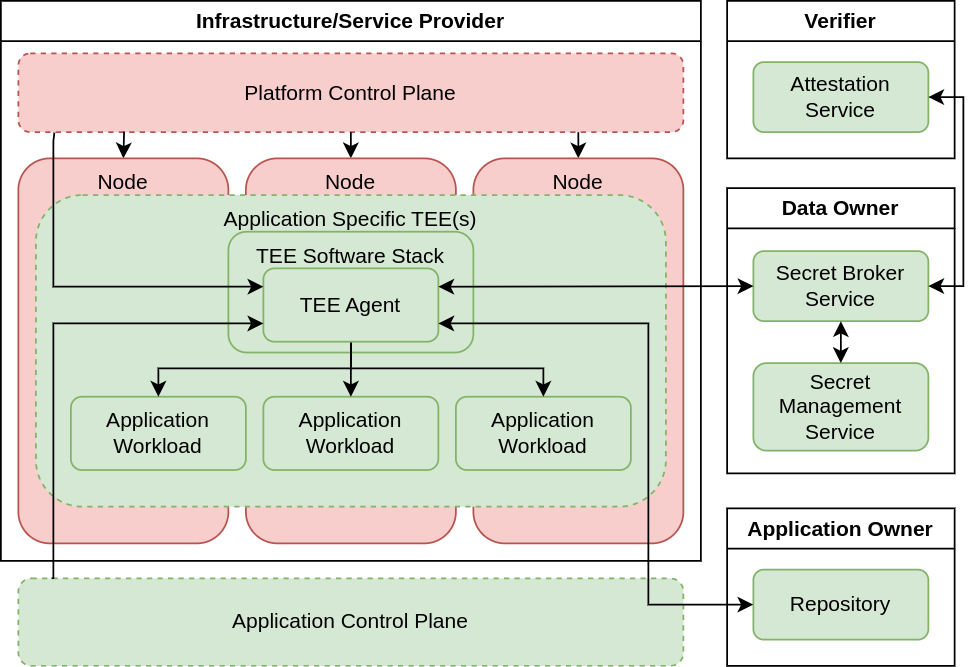
\includegraphics{resources/architecture-overview.png}
  \caption[A simplified overview over the Confidential Containers architecture]{
    An overview over components used in this architecture proposal. Defines
    which components are managed by which role and whether it is trusted.
    Entities and Components marked in red are untrusted, while those marked in
    green are trusted.}
  \label{fig:confidential-containers-overview}
\end{figure}

Figure \ref{fig:confidential-containers-overview} shows an overview over the
components used in this architecture proposal. The next sections explain these
components, their responsibilities, and the managing role.

\subsection{Components}

\subsubsection{Control Planes}

In a dynamically provisioned platform managing the infrastructure and
orchestrating applications is the responsibility of the control plane. We are
grossly simplifying the control plane here by considering it as a single
component. In traditional platforms the control plane is a high-privileged
component in order to perform management and orchestration tasks.

We want to apply the least privileges principle to the control plane and only
allow privileges necessary for basic management and orchestration. This includes
managing the lifecycle of applications on a node, migration of applications
between nodes, and monitor computing resource usage. But privileges that have
the potential to compromise the integrity of application code and data should
only be assigned to trusted entities and components. This implies that entities
and components controlled by the service provider should not have these
privileges.

To achieve this the traditional control plane has to be split

\subsubsection{Enclave Agent}

\subsubsection{Repository}

\subsubsection{Secrets Broker Service}

\subsubsection{Secrets Management Service}

\subsubsection{Attestation Service}
